\documentclass[tikz]{standalone}

\usepackage[latin1]{inputenc}
\usepackage{tikz}

% GNUPL
\begin{document}

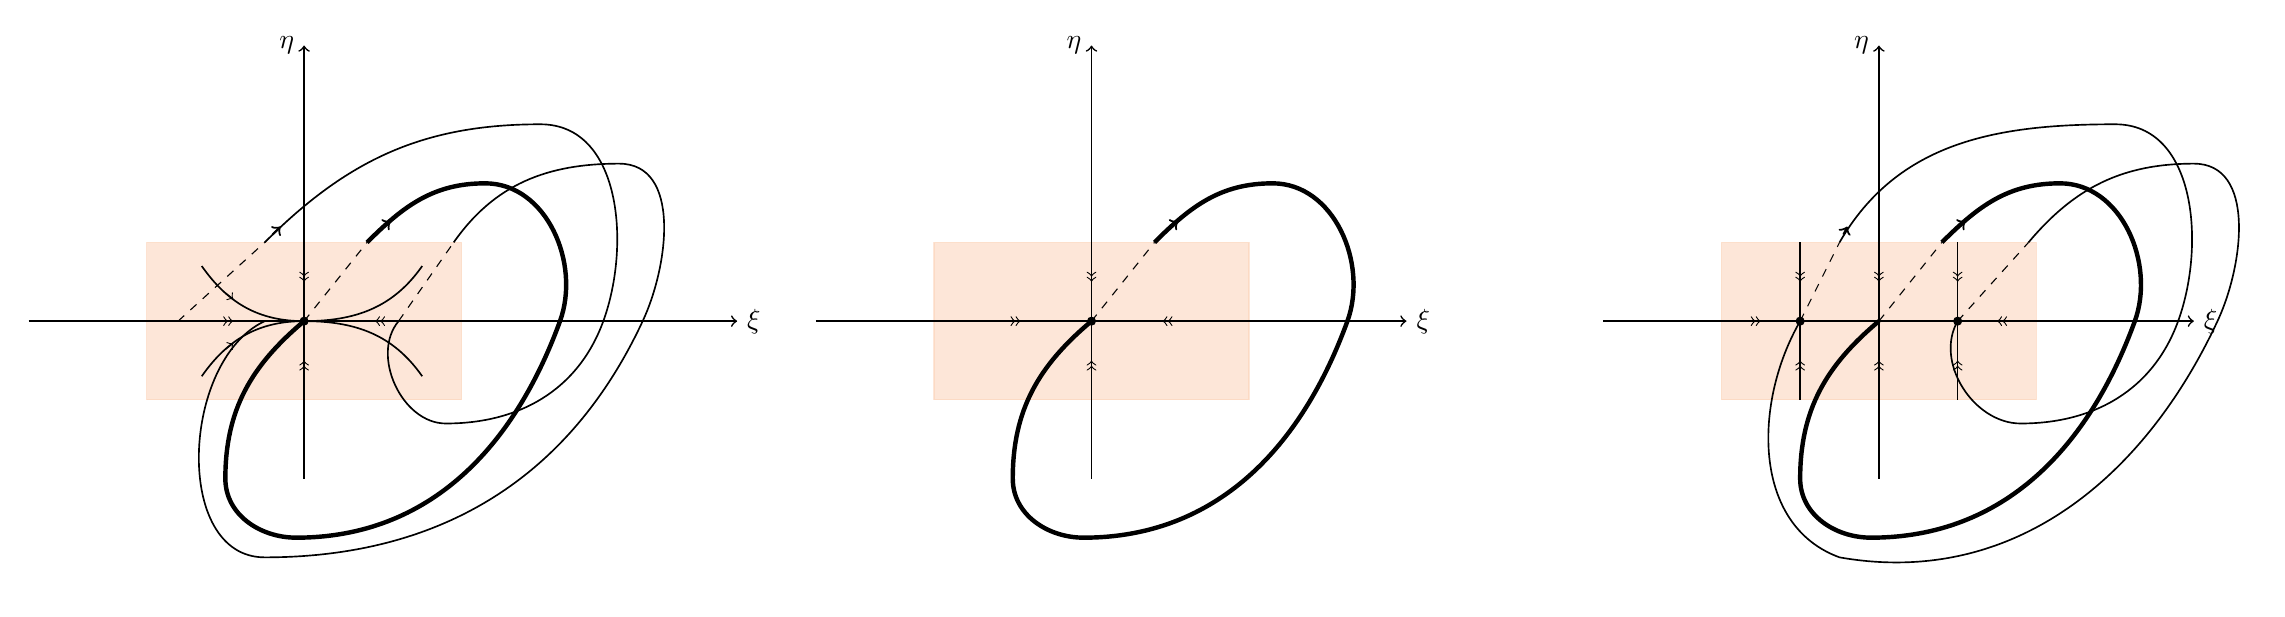
\begin{tikzpicture}
    %\mu<0
    \draw[color={rgb,255:red,251; green,206; blue,177}, opacity=0.2][fill, opacity=0.5] (2,3) --(6,3)--(6,5) --(2,5)--(2,3);
    \draw[semithick] [->] (0.5,4) -- (9.5,4) node[right] {$\xi$};
    \draw[semithick] [->] (4,2) -- (4,7.5) node[left] {$\eta$};
    \draw[->>] (4,4.6) --(4,4.5);
    \draw[->>] (4,3.4) --(4,3.5);
    \draw[->>] (3,4) --(3.1,4);
    \draw[->>] (5,4) --(4.9,4);
    \draw [fill] (4,4) circle [radius=0.05];
    \draw[semithick] (2.7,4.7) to [out=-55,in=180] (4,4);
    \draw[semithick] (2.7,3.3) to [out=55,in=180] (4,4);
    \draw[semithick] (5.5,3.3) to [out=125,in=0] (4,4);
    \draw[semithick] (5.5,4.7) to [out=-125,in=0] (4,4);
    \draw[->] (3,4.36) --(3.1,4.28);
    \draw[->] (3,3.64) --(3.1,3.72);
    \draw[dashed] (4,4) --(4.8,5);
    \draw[ultra thick] (4.8,5) to [out=45,in=180] (6.3,5.75) to [out=0,in=70] (7.25,4) to [out=-110,in=0] (3.9,1.25) to [out=180,in=-90] (3,2) to [out=90,in=-140] (4,4);
    \draw[thick] [->] (5,5.2) --(5.1,5.27);
    \draw[dashed] (2.4,4) --(3.5,5);
    \draw[semithick] (3.5,5) to [out=45,in=180] (7,6.5) to [out=0,in=70] (7.8,4) to [out=-110,in=0] (5.8,2.7) to [out=180,in=-130] (5.2,4);
    \draw [dashed] (5.2,4) --(5.9,5);
    \draw[semithick] (5.9,5) to [out=55,in=180] (8,6) to [out=0,in=65] (8.3,4) to [out=-115,in=0] (3.5,1) to [out=180,in=-155] (3.5,4);
    \draw[thick] [->] (3.6,5.1) --(3.7,5.2);

	%\mu=0
    \draw[color={rgb,255:red,251; green,206; blue,177}, opacity=0.2][fill, opacity=0.5] (12,3) --(16,3)--(16,5) --(12,5)--(12,3);
    \draw[semithick] [->] (10.5,4) -- (18,4) node[right] {$\xi$};
    \draw[semithick] [->] (14,2) -- (14,7.5) node[left] {$\eta$};
    \draw[->>] (14,4.6) --(14,4.5);
    \draw[->>] (14,3.4) --(14,3.5);
    \draw[->>] (13,4) --(13.1,4);
    \draw[->>] (15,4) --(14.9,4);
    \draw[dashed] (14,4) --(14.8,5);
    \draw[ultra thick] (14.8,5) to [out=45,in=180] (16.3,5.75) to [out=0,in=70] (17.25,4) to [out=-110,in=0] (13.9,1.25) to [out=180,in=-90] (13,2) to [out=90,in=-140] (14,4);
    \draw[thick] [->] (15,5.2) --(15.1,5.27);
    \draw [fill] (14,4) circle [radius=0.05];
    %\mu>0
    \draw[color={rgb,255:red,251; green,206; blue,177}, opacity=0.2][fill, opacity=0.5] (22,3) --(26,3)--(26,5) --(22,5)--(22,3);
    \draw[semithick] [->] (20.5,4) -- (28,4) node[right] {$\xi$};
    \draw[semithick] [->] (24,2) -- (24,7.5) node[left] {$\eta$};
    \draw[->>] (24,4.6) --(24,4.5);
    \draw[->>] (24,3.4) --(24,3.5);
    \draw[->>] (22.4,4) --(22.5,4);
    \draw[->>] (25.6,4) --(25.5,4);
    \draw[semithick] (23,5) -- (23,3);
    \draw[semithick] (25,5) -- (25,3);
    \draw[->>] (23,4.6) --(23,4.5);
    \draw[->>] (23,3.4) --(23,3.5);
    \draw[->>] (25,4.6) --(25,4.5);
    \draw[->>] (25,3.4) --(25,3.5);
    \draw[dashed] (24,4) --(24.8,5);
    \draw[ultra thick] (24.8,5) to [out=45,in=180] (26.3,5.75) to [out=0,in=70] (27.25,4) to [out=-110,in=0] (23.9,1.25) to [out=180,in=-90] (23,2) to [out=90,in=-140] (24,4);
    \draw[thick] [->] (25,5.2) --(25.1,5.27);
    \draw[dashed] (23,4) --(23.5,5);
    \draw[semithick] (23.5,5) to [out=60,in=180] (27,6.5) to [out=0,in=70] (27.8,4) to [out=-110,in=0] (25.8,2.7) to [out=180,in=-120] (25,4);
    \draw [dashed] (25,4) --(25.9,5);
    \draw[semithick] (25.9,5) to [out=50,in=180] (28,6) to [out=0,in=65] (28.3,4) to [out=-115,in=-10] (23.5,1) to [out=-200,in=-120] (23,4);
    \draw[thick] [->] (23.55,5.1) --(23.6,5.2);
    \draw [fill] (25,4) circle [radius=0.05];
    \draw [fill] (23,4) circle [radius=0.05];

\end{tikzpicture}


\end{document}